%\section{Linux API Study}
%\label{sec:syspop:study}

%\note{about 3 pages, include graphs}
%\note{try to break the page here so the whole observation can start on a new page}

%This section presents measurements of API usage,
%as well as several trends in how APIs are used. Of particular note is that
%the OS interface required by essentially all applications is 
%%the total OS interface that essentially all applications require is
%substantially larger than the roughly 300 Linux system calls---the required interface
%also includes several vectored system call operations, such as {\tt ioctl}, and special filesystem interfaces like {\tt /sys} and {\tt /proc}.
%We also note that a number of system calls and other APIs are so rarely used that they can be deprecated with little disruption or effort.
%
%This section first examines the use of system calls in Linux applications.
%Section~\ref{sec:observation:hello} analyzes the most efficient path to add system calls
%to a prototype, outlining a path from the minimal footprint for ``hello world'', 
%up through the most demanding application (qemu), maximizing the number
%of supported applications at each step.
%Section~\ref{sec:observation:vector} analyzes the importance of operations
%under vectored system calls, such as {\tt ioctl}.
%Section~\ref{sec:observation:pseudo} evaluates the \usagemetric{} of 
%pseudo-files, such as those under {\tt /proc}.
%Finally, Section~\ref{sec:observation:libc}
%examines current usage patterns for \libc{}.
%Throughout the section, we identify several points at which APIs could be gainfully
%restricted, removed, or refactored,
%as well as identifying points where unexpected APIs can be essential to performance or
%functionality.
%We highlight key insights and recommendations in boxes.

%% \rev{Explain the structure.}{In the following subsections,
%% we will discuss our findings on the API usage of different interface types,
%% followed by %boxed take-aways our quick tips (in double-framed boxes)
%% the lessons or insights in boxes.} 
%% \fixmedp{If a reviewer asked for a structure, I expect they want to know something like:
%% We first present system calls, then ioctls,
%% then pseudo file systems, etc.  In other words, what is the organizing principle for 
%% the following sub-sections?  Not that we discuss and then have a box} 

%\subsection{\usagemetric{} of Linux System Calls}
\section{Linux system calls}
\label{sec:study:syscall}

%We begin by looking at the \usagemetric{} of each system call, 
%ordered by total application installations and regularly used applications 
%in order to answer the following questions:
%\begin{compactitem}
%\item Which system calls are the most important to support when implementing a new system,
%or have high costs to replace, if desired?
%%1) do we definitely need to support any of the surveyed systems?
%%2) are used by at least one frequently used application on the surveyed systems?
%\item Which system calls are very rarely used and candidates for deprecation?
%\item Which system calls are not supported by the OS, but still attempted by applications?
%\end{compactitem}
%\vspace{10pt}

There are \syscallnum{} system calls defined in \osarch{} Linux \kernelversion{} (as listed in {\tt unistd.h}). 
Figure~\ref{fig:syscall-popularity-trend} shows the 
distribution of system calls by importance.
The Figure is ordered by most important (at 100\%) to least important (around 0\%)---similar
to inverted CDF.
The figure highlights several points of interest on this line.

%The trends \byinst{} are useful to answer questions about supporting complete installations, 
%while the trends \byvote{} are useful to answer questions about supporting most popular 
%applications on most of the systems.
Over two-thirds ({\em 224 of \syscallnum{}}) 
of system calls on Linux are indispensable:
required by 
at least one application on every installation.
%only a little 
%over one-thirds ({\em 121 of \syscallnum{}}) of system calls are required 
%by at least one regularly used application (\byvote{}).
%\fixmedp{Would be nice to have more to say here, like filling out weighted compliance and the number of packages}
Among the rest, 33 system calls are important on more than ten percent of the installations.
44 system calls have very low \usagemetric{}:
less than ten percent of the installations include at least one application
that uses these system calls.
%Moreover, less than 10\% of the systems require 43 system calls.
%and 58 system calls are regularly used on less than 10\% of the systems (\byvote{}).
%For instance, {\tt timer\_delete}, {\tt timer\_create} and {\tt timer\_settime} are used by 
%at least one application on all the systems, however, the applications using these 
%system calls are regularly used only on 17\% of the systems. 
%Another system call 
%{\tt tkill} used by {\tt strace} installed ubiquitously on all systems 
%is used regularly only on 3\% of the systems. So, even if the installation statistics imply that 
%{\tt tkill} needs to be supported to support at least one of the machines,
%only 3\% of those machines regularly use that system call.

Our study also shows the contributors
to an API's importance. %\usagemetric{}.
For instance, Table~\ref{tab:syspop:wrapped} lists system calls that are
only called by one or two particular libraries
(e.g., \libc{}).
These system calls are wrapped by library APIs,
so applications depend on them only because the libraries do.
To eliminate the usage of these system calls,
developers only have to pay minimum efforts to re-implement the wrappers in libraries.

\begin{figure}[t]
\centering
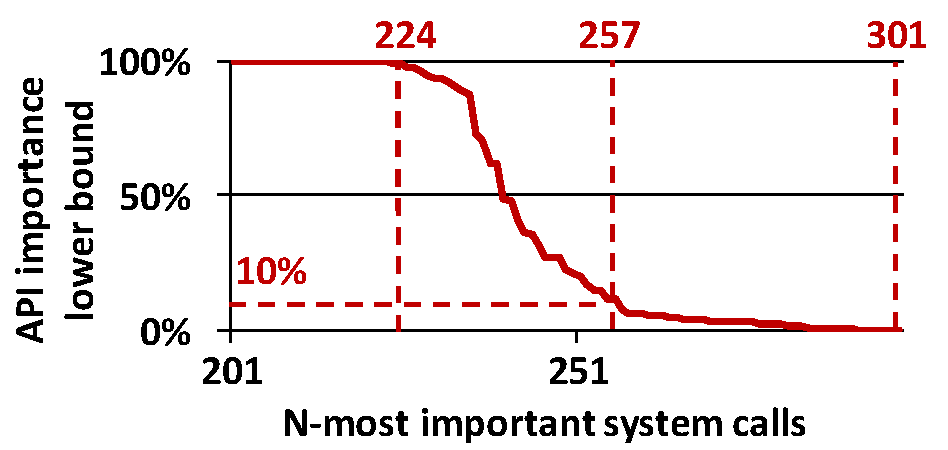
\includegraphics[width=\textwidth]{syscall-popularity-all-by-inst.pdf}
\caption[N-most important system calls in Linux.]
{The trend of \usagemetric{} as N-most important system calls among total \syscallnum{} system calls of \osversion{} with Linux kernel \kernelversion{}. .
Higher is more important; 100\% indicates all installations include software that make the system call.}
\label{fig:syscall-popularity-trend}
\end{figure}

%\callout{It is easy to support regularly used parts of an installation than complete installations of the surveyed systems.} 

Among the 44 system calls with a \usagemetric{} above zero but less than ten percent,
some are cases where a more popular alternative is available.
%developers appear more motivated by 
%portability than security.
%, the bottom 20 non-zero are listed in Table~\ref{tab:syscall-popularity-bottom}, along with the packages that use these interfaces.
%%11 of the bottom 20 system calls are Linux-specific.
%%This shows that portability to other Unix variants
%%has a significant effect on adoption.
%%bP: These conclusions cannot be made with weighted importance.
For instance, Linux supports both POSIX and System V message queues.
The five APIs for POSIX message queues have a lower
\usagemetric{} than System V message queues.
We believe this is attributable to System V message queues %provide a better designed interface, they
being more portable to other UNIX systems.
%they are not adopted by most popular applications.}
Similarly, we observed that {\tt epoll\_wait} (100\%) has a higher \usagemetric{} than {\tt epoll\_pwait} (3\%),
even though {\tt epoll\_pwait} is commonly considered more robust
for the same purpose---waiting on file descriptor events.
Table~\ref{tab:dominated} lists
system calls used by only one or two packages---generally special-purpose utilities,
such as {\tt kexec\_load}, which is used by {\tt kexec-tools}).
%,These system calls are mostly used by special-purpose utilities (e.g., 
%and generally address  because their semantics are not friendly enough.

\begin{table}[t!b!]
  \centering
  \small
  \begin{tabular}{>{\footnotesize\raggedright\arraybackslash}p{1.45in} >{\raggedleft\arraybackslash}p{0.25in}>{\raggedright\arraybackslash}p{1.15in}}
\toprule
{\bf System Calls} & {\bf Imp.} & {\bf Packages}\\
\midrule
{\tt clock\_settime}, {\tt iopl}, {\tt ioperm},  {\tt signalfd4}  & 100\% & libc \\
{\tt mbind}             & 36.0\% & libnuma, libopenblasp \\
{\tt addkey}            & 27.2\% & libkeyutils \\
{\tt keyctl}            & 27.2\% & pam\_keyutil, libkeyutils \\
{\tt requestkey}        & 14.4\% & libkeyutils \\
{\tt preadv}, {\tt pwritev}   & 11.7\% & libc \\
    \end{tabular}%
   \caption{System calls which are only directly used by particular libraries, and their \usagemetric{} (``Imp.''). Only system calls with \usagemetric{} larger than ten percent are shown.
These system calls are wrapped by library APIs,
thus they are easy to deprecate by modifying the libraries.  
}
  \label{tab:wrapped}%
\end{table}%

\begin{table}[t!b!]
\centering
\small
\begin{tabular}{>{\palign[\footnotesize]{l}}p{2.9in} >{\palign{r}}p{1.1in}>{\palign{l}}p{2in}}
\toprule
{\bf System Calls} & {\bf \UsageMetric{}} & {\bf Used Packages}\\
\midrule
{\tt seccomp}, {\tt sched\_setattr}, {\tt sched\_getattr}  & 1\% & coop-computing-tools \\
\hline
{\tt kexec\_load} & 1\% & kexec-tools \\
\hline
{\tt clock\_adjtime} & 4\% & systemd \\
\hline
{\tt renameat2} & 4\% & systemd, coop-computing-tools \\
\hline
{\tt mq\_timedsend}, {\tt mq\_getsetattr} & 1\% & qemu-user \\
\hline
{\tt io\_getevent} & 1\% & ioping, zfs-fuse \\
\hline
{\tt getcpu} & 4\% & valgrind, rt-tests \\
\hline
\end{tabular}%
\caption[System call usage dominated by particular package(s)]
{System calls with usage dominated by particular package(s), and their \usagemetric{}. This table excludes system calls that are officially retired.}
\label{tab:dominated}%
\end{table}%


In some cases, system calls are effectively offloaded to a file in {\tt /proc} or {\tt /sys}.
For instance, some of the information that was formerly available via 
{\tt query\_module} can be obtained from {\tt /proc/modules}, {\tt /proc/kallsyms} 
and the files under the directory {\tt /sys/module}. Similarly, the information that can be obtained from the {\tt sysfs} system call
is now available in {\tt /proc/filesystems}.

%We found five  API that have very low 
%compared to the System V message queue API.

We also found five system calls {\tt uselib}, {\tt nfsservctl}, {\tt afs\_syscall}, {\tt vserver} and {\tt security} system calls that are officially retired, but still have a low, but non-zero, \usagemetric{}. 
For instance {\tt nfsservctl} is removed from Linux kernel 3.1 but
still has \usagemetric{} of seven percent,  %\fixmedp{Do we have some examples of apps that use it?}
because it is tried by NFS utilities such as {\tt exportfs}.
These utilities still attempt the old calls for backward-compatibility with older kernels.
%Application maintainers of packages using these retired system calls need to be notified to port their applications to support latest kernel.


%\callout{System developers can use our framework to actively notify relevant package maintainers while retiring system calls.} 
%\callout{Among 43 least-used system calls, some are replaceable
%by alternatives with higher \usagemetric{};
%5 are officially retired but still tried by few applications.
%System developers could use this data to identify relevant applications,
%accelerating replacement of these system calls.}




\begin{table}[t!b!]
\centering
\small
\begin{tabular}{>{\palign[\footnotesize]{l}}p{.5\textwidth} >{\palign{l}}p{.45\textwidth}}
\toprule
\textbf{Unused System Calls} & \textbf{Reason for Disuse}\\
\midrule
{\footnotesize
{\tt set\_thread\_area}, {\tt tuxcall}, {\tt create\_module}, and 7 more. } & Officially retired.\\
\hline
{\tt sysfs} & replaced by {\tt /proc/filesystems}.\\
\hline
{\tt rt\_tgsigqueueinfo}, {\tt get\_robust\_list} & Unused by applications.\\
\hline
{\tt remap\_file\_pages} & No non-sequential ordered mapping; repeated calls to mmap preferred.\\
\hline
{\tt mq\_notify} & Unused: Asynchronous message delivery.\\
\hline
{\tt lookup\_dcookie} & Unused: for profiling.\\
\hline
{\tt restart\_syscall} & Transparent to applications.\\
\hline
{\tt move\_pages} & Unused: for NUMA usage. \\
\hline
\end{tabular}%
\caption{Unused system calls and explanation for disuse.}
\label{tab:syspop:unused}%
\end{table}%



%On the other end of the spectrum, 

In total, 18 of \syscallnum{} system calls in Linux \kernelversion{} are not used by any application in the \osdist{} repository. We list these system calls in Table~\ref{tab:syspop:unused}.
In addition to the issues discussed above,
Ten of these system calls do not have an entry point, but are still defined in the Linux headers.
%\fixmedp{Why are they in the count then?  do you mean 320 defined system call numbers}
%Similarly, we analyze the 21 system calls with 0 \usagemetric{} as shown in 
%Table~\ref{tab:unused}. 
%{\tt sysfs} is replaced by alternate interface {\tt /proc/file\linebreak[0]systems}.
%%On the other hand, even though {\tt remap\_file\_pages} system call was added to map pages of a file into memory in a non-sequential order since Linux version 2.6 (in 2003), no application is actually using it. This indicates that either no application is mapping pages in non-sequential order or applications are repeatedly using the more popular generic system call like {\tt mmap}.
%Similarly, {\tt mq\_notify} system call for receiving asynchronous notification about new messages in message queue is not used, because \usagemetric{} of message queue interfaces is less than 5\% in the first place and applications using message queue do not use asynchronous communication.
Five of the unused system calls such as {\tt rt\_tgsig\linebreak[0]queueinfo}, {\tt get\_robust\_list}, {\tt remap\_\linebreak[0]file\_pages}, {\tt mq\_notify}, {\tt lookup\_dcookie} provide an interface that is not used by the applications. These system calls can be potential candidates for deprecation.
However, even though {\tt restart\_\linebreak[0]syscall} is not used by any application, it is internally used by the kernel. % transparent to userspace.
%Finally, 4 NUMA related system calls are not used 
%\rev{rewrite}{because none of our samples is written to be NUMA-aware}.
%\fixmetsai{Check if libnuma uses these system calls.}

%\callout{In addition to ten already retired system calls, we found seven other candidate system calls for deprecation or in need of more exposure to developers.}

\begin{comment}
\begin{table}[t]
\center{
\footnotesize
\begin{tabular}{m{0.45\linewidth}m{0.45\linewidth}}
\hline
Syscalls & Packages\\
\hline
process\_vm\_writev & coop-computing-tools, care, proot, stress-ng \\
vserver & util-vserver\\
syncfs & ceph-test, ploop, ruby-passenger, ceph\\
io\_getevents & ioping, zfs-fuse\\
uselib & mupdf, mupdf-tools\\
afs\_syscall & openafs-fileserver, openafs-kpasswd, openafs-krb5, openafs-client, openafs-dbserver\\
kexec\_load & kexec-tools\\
mq\_getsetattr, mq\_timedsend & qemu-user, qemu-user-static\\
vmsplice & criu, qemu-user-static, fio, stress-ng, qemu-user\\
timer\_gettime & ben, galax-extra, libocamlnet-ocaml-bin, ocsigenserver, galax, approx, qemu-user-static, galaxd, matita, cduce, qemu-user, turnserver, stress-ng\\
timerfd\_gettime & ben, approx, libocamlnet-ocaml-bin, ocsigenserver, openclonk, matita, galax, galaxd, qemu-user-static, galax-extra, cduce, qemu-user\\
eventfd & blktap-utils, julia, nodejs\\
semtimedop & tgt, dahdi, gtk-gnutella, prayer, libopenni-sensor-primesense0, libopenni-sensor-pointclouds0\\
timer\_getoverrun & emacs24-lucid, emacs24, qemu-user-static, qemu-user, emacs24-nox, rt-tests, reconserver, miredo\\
mq\_timedreceive & qemu-user-static, nilfs-tools, xjadeo, rt-tests, qemu-user\\
acct & watchdog, acct, qemu-user-static, qemu-user, scm, atop\\
fanotify\_init, fanotify\_mark & fatrace, fnotifystat, health-check, clamav-daemon\\
open\_by\_handle\_at & qemu-system-mips, qemu-system-misc, qemu-system-sparc, qemu-system-ppc, qemu-system-arm, qemu-system-x86\\
\hline
\end{tabular}
}
\footnotesize
\caption{20 system calls with the lowest \usagemetric{} among 297 used system calls in \osversion{} with Linux Kernel \kernelversion{}, except the ones with \usagemetric{} lower than 0.01\% (considered negligible).}
\label{tab:syscall-popularity-bottom}
\end{table}
\end{comment}

\begin{comment}
There are 43 system calls with low non-zero \usagemetric{} of less than 10\%.
%, the bottom 20 non-zero are listed in Table~\ref{tab:syscall-popularity-bottom}, along with the packages that use these interfaces.
%%11 of the bottom 20 system calls are Linux-specific.
%%This shows that portability to other Unix variants
%%has a significant effect on adoption.
%%bP: These conclusions cannot be made with weighted importance.
We found 5 POSIX message queue API that have very low 
\usagemetric{} compared to the System V message queue API because 
even if POSIX message queues provide a better designed interface, they are less 
widely available. We also found 5 system calls {\tt uselib}, {\tt nfsservctl}, {\tt afs\_syscall}, {\tt vserver} and {\tt security} system calls that are officially retired, and have non-zero albeit negligible \usagemetric{}. 
For instance {\tt nfsservctl} is removed from Linux kernel 3.1 but
still has \usagemetric{} of 7\%. Application maintainers of packages using these retired system calls need to be notified to port their applications to support latest kernel.
Also, we observed that {\tt epoll\_wait} (100\%) has more \usagemetric{} than {\tt epoll\_pwait} (3\%)
even though {\tt epoll\_pwait} is safer to use to wait for a file descriptor to become available.
In some cases, system calls are effectively offloaded to a file in {\tt /proc} or {\tt /sys}.
For instance, some of the information that was formerly available via 
{\tt query\_module} can be obtained from {\tt /proc/modules}, {\tt /proc/kallsyms} 
and the files under the directory {\tt /sys/module}. Also same information obtained from {\tt sysfs} is
also available from {\tt /proc/filesystems}.

\callout{System developers can use our framework to actively notify relevant package maintainers while retiring system calls.} 
\end{comment}

%%% \begin{figure}[H]
%%% \center{
%%% \includegraphics[height=1.1in]{figures/syscall-popularity-top-1.pdf}
%%% \hspace{-0.3in}
%%% \includegraphics[height=1.1in]{figures/syscall-popularity-top-2.pdf}
%%% }

%%% \begin{minipage}[t]{\linewidth}
%%% \scriptsize
%%% \vspace{-0.1in}
%%% \setlength{\parindent}{-0.2in}
%%% \setlength{\leftskip}{0.2in}
%%% {\bf * Top-1:} \hspace{0.1in}(195 system calls) \hspace{0.1in}\usagemetric{} = 1.0000\\
%%% {\tiny\tt
%%% read,write,open,close,stat,polllseek,mmap,brk,rt\_sigprocmask,ioctl,access,pipe,select,shmget,nanosleep,socket,clone,vfork,kill,
%%% etc.
%%% }

%%% \vspace{0.1in}
%%% {\bf * Top-2:} \hspace{0.1in}(8 system calls) \hspace{0.1in}\usagemetric{} = 0.9999\\
%%% {\tiny\tt
%%% reboot,timer\_create,iopl,getitimer,accept4,
%%% etc.
%%% }
%%% \end{minipage}
%%% \footnotesize
%%% \caption{20 groups of system calls with the highest \usagemetric{} among 279 used system calls in \osversion{} (Linux Kernel \kernelversion{})}
%%% \label{fig:syscall-popularity-top}
%%% \end{figure}

%\begin{figure}[H]
%\center{
%\includegraphics[height=1.15in]{figures/syscall-popularity-bottom.pdf}
%}
%\footnotesize
%\caption{20 system calls with the lowest \usagemetric{} among 279 used system calls in \osversion{} (Linux Kernel \kernelversion{}), except the ones with \usagemetric{} lower than 0.0001 (considered negligible).\fixmedp{Convert to table}}
%\label{fig:syscall-popularity-bottom}
%\end{figure}

%\subsection{From ``Hello World'' to Qemu}
%\label{sec:observation:hello}

Figure~\ref{fig:syscall-compatibility} shows the optimal path of adding system calls to a prototype system,
using a simple, greedy strategy of implementing the N-most important APIs, which in turns
maximizes \compatmetric{}.
In other words, the leftmost points on the graph are the most important APIs,
but the y coordinate only increases once enough system calls
are supported that a simple program, such as ``hello world'' can execute. %\fixmedp{Right?}
Similar to a CDF, this line
continues up to 100\% of Ubuntu applications.  The graph highlights several 
points of interest in this curve.

Essentially, one cannot run even the most simple programs without at least 40 system calls.
After this, the number of additional applications one can support by adding another system call increases
steadily until an inflection point at 125 system calls, or supporting extended attributes on files,
where \compatmetric{} jumps to 25\%.
To support roughly half of \osdist{} applications, one must have 145 system calls, and
the curve plateaus around 202 system calls.  
On the most extreme end, qemu's MIPS emulator (on an \osarch{} host) requires 270 system calls~\citep{Bellard05}.
A \compatmetric{} of 100\% implies that
%all Linux system calls
all Linux applications ever used
are supported by the prototype.

\begin{figure}[t]
\centering
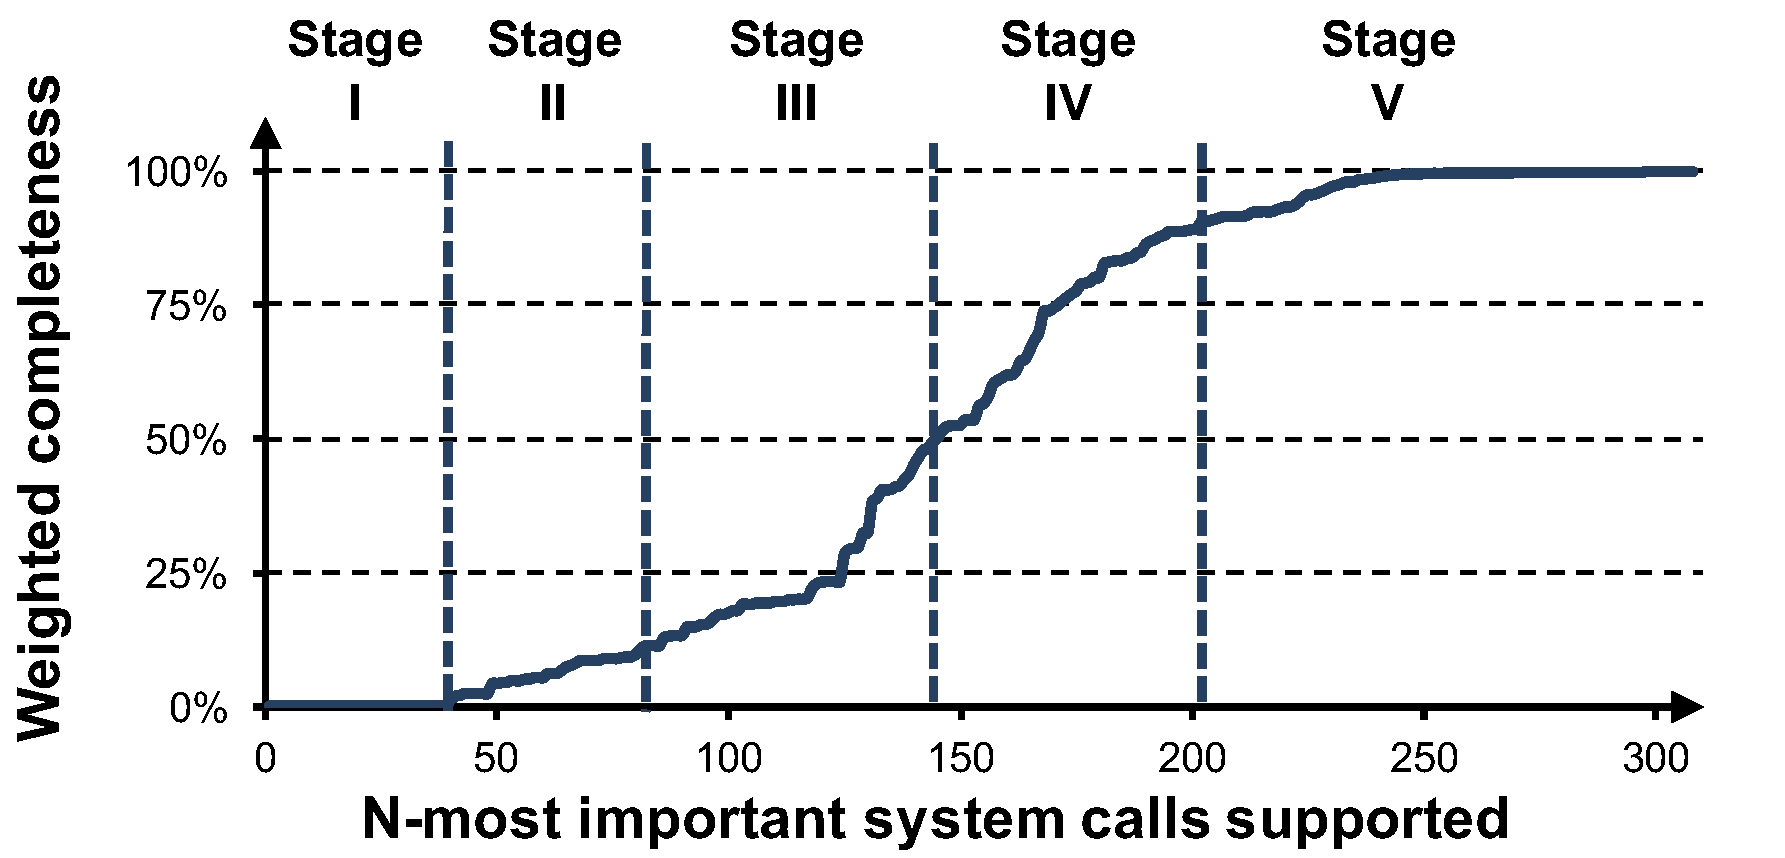
\includegraphics[width=.8\textwidth]{syscall-compatibility.pdf}
\caption{Accumulated \compatmetric{} when N top-ranked system calls are implemented in the OS. Higher is more compliant.}
\label{fig:syscall-compatibility}
\end{figure}

\begin{table}[t]
\center{
\begin{tabular}{c>{\footnotesize\raggedright\arraybackslash}m{.5\textwidth}>{\raggedleft}m{.15\textwidth}>{\raggedleft\arraybackslash}m{.15\textwidth}}
\toprule
Stage & {\normalsize Sample System Calls} & \# syscalls & {\footnotesize \CompatMetric{}} \\
\addlinespace
\midrule
I &
{\tt mmap}, {\tt vfork}, {\tt exit}, {\tt read},
{\tt gettid}, {\tt fcntl}, {\tt getcwd}
{\tt sched\_yield}, {\tt kill}, {\tt dup2}
& 40 & 1.12 \% \\
\midrule
II &
{\tt mremap}, {\tt ioctl}, {\tt access}, {\tt socket},
{\tt poll}, {\tt recvmsg}, {\tt dup},
{\tt unlink}, {\tt wait4}, {\tt select}, {\tt chdir}, {\tt pipe}
& +41 (81) & 10.68 \% \\
\midrule
III &
{\tt sigaltstack}, {\tt shutdown}, {\tt symlink},
{\tt alarm}, {\tt listen}, {\tt pread64}, {\tt getxattr}, 
{\tt shmget}, {\tt epoll\_wait},
{\tt chroot}
& +64 (145) & 50.09 \% \\
\midrule
IV &
{\tt flock}, {\tt semget}, {\tt ppoll},
{\tt mount}, {\tt brk}, {\tt pause},
{\tt clock\_gettime}, {\tt getpgid}, {\tt settimeofday},
{\tt capset}
& +57 (202) & 90.61 \% \\
\midrule
V & {\normalsize All remaining} & +70 (272) & 100 \% \\
\bottomrule
\end{tabular}
}
\footnotesize
\caption[Proposed steps of Linux system call implemetation prioritzed by importance]
{Five stages of implementing system calls based on the \usagemetric{} ranking. For each stage, a set of system calls is listed, with the work needed to accomplish (\# of system calls) and the \compatmetric{} that can be reached.}
\label{tab:syscall-stage}
\end{table}

Table~\ref{tab:syscall-stage} breaks down the recommended development phases by rough categories of required system calls.
We do not provide a complete ordered list here in the interest of brevity, but this list is available as part of our dataset, 
at \projecturl{}.

A goal of \compatmetric{} is to help guide the process of developing new system prototypes.
Section~\ref{sec:study:syscall} showed that 224 out of \syscallnum{} system calls on \osdist{} have 100\% \usagemetric{}.
In other words, if one of these 224 calls is missing, at least one application on a typical system will not work.
\Compatmetric{}, however, is more forgiving, as
it tries to capture the fraction of a typical installation that could work.
Only 
40 system calls are needed to have \compatmetric{} more than 1\%.
%However, to achieve non-zero \compatmetric{} to \osdist{}, it does not require a system to support all 226 system calls;
%only 
%% The reason of such a gap is that \usagemetric{} is
%% a metric more sensitive to the API usage of individual applications:
%% as long as at least one application in every installation uses
%% a specific API, its \usagemetric{} will be 100\%.
%% \compatmetric{} is a metric made relatively relaxed:
%% this metric evaluates the expected fraction of any installation that can be supported,
%% to provide meaningful measurements

%\callout{It takes the most effort to support first and last 10\%
%of any installation (0--10\% and 90--100\% \compatmetric{}).
%The gain in functionality is precipitous when adding the 81st--202nd system calls.}

For simplicity, Table~\ref{tab:syscall-stage}
only includes system calls, % \compatmetric{} based on system ,
but one can construct a similar path including other APIs, % the metric also considers other APIs,
such as vectored system calls, pseudo-files and library APIs.
For example, developers need not implement every operation of
{\tt ioctl}, {\tt fcntl} and {\tt prctl}
during the early stage of developing a system prototype.
%\fixmedp{Would it make sense to do this after the ioctls and files are covered, and include important ioctls and files?  Also, check my rewrite}

%\fixmedp{This callout is not really justified by the text  I took the point to be that the right 132 and 202 system calls are ``sweet spots'' on the path to maturity.}

\section{Vectored system call opcodes}
\label{sec:study:opcodes}

%\fixmedp{I think RD is right: can we give more landscape of what the long tail of vectored calls are for?  Why do they exist?}

Some system calls, such as {\tt ioctl}, {\tt fcntl},
and {\tt prctl}, essentially export a secondary system call table, 
using the first argument as an operation code.
These {\it vectored} system calls significantly expand the system API, 
dramatically increasing the effort to realize full API compatibility.
%and essentially make it harder to implement a compatibility layer.
It is also difficult to enforce robust security policies on these interfaces,
as the arguments to each operation are highly variable.
%\fixmedp{Can we comment on what, say SELinux or AppArmor actually do with ioctl?}


The main expansion is from {\tt ioctl}.
Linux defines 635 operation codes, and 
Linux kernel modules and drivers can define additional operations.
In the case of {\tt ioctl}, we obverse that there are 52 operations with the 100\% \usagemetric{} (Figure~\ref{fig:syspop:opcode-popularity}),
each of which are as important as the 226 most important system calls.
Of these 52 operations,  47 are frequently used operations for TTY console (e.g., {\tt TCGETS}) or generic operations on IO devices (e.g., {\tt FIONREAD}).

%A narrow vectored system call like {\tt fcntl} has eighteen operations in , and {\tt prctl} has 44 operations so far.
%A wider vectored system call like 
%which are further 



On the narrow end, {\tt fcntl} and {\tt prctl} have 18 and 44 operations, respectively, in Linux kernel \kernelversion{}.
Unlike {\tt ioctl}, {\tt fcntl} and {\tt prctl} are not extensible by modules or drivers,
and their operations tend to have higher \usagemetric{} (Figure~\ref{fig:syspop:opcode-popularity}).
For {\tt fcntl}, eleven out of eighteen {\tt fcntl} operations in Linux \kernelversion{} have \usagemetric{} at around 100\%.
For {\tt prctl}, only nine out of 44 operations have \usagemetric{} around 100\%,
and only eighteen has \usagemetric{} larger than 20\%.
%Because of the more equally important operations, {\tt fcntl} is a less urgent target for reformation, while {\tt prctl} has plenty of unused or infrequently used read-only operations that can be moved to pseudo-file system interfaces like {\tt /proc}.


Thus, developers of a new system prototype should support these 47 most important {\tt ioctl}
operations, about half of the {\tt fcntl} opcodes, and only 9--20 {\tt prcntl} operations.


%% Although the 47-most important ioctl operations have 100\% \usagemetric{},
%% promoting any of these operations to system calls is not beneficial.
%% Vectored system calls with limited amounts of operation codes
%% are almost equally easy to secure and maintain
%% as normal system calls.
%% However the disruptiveness of removing these operations codes
%% is unbearable for applications. 

%% However, knowing the most important operations for vectored system calls,
%% developers of new system prototypes can choose to
%% implement only part of these vectored system calls to obtain significant improvement on \compatmetric{}.
%% %For instance, Graphene library OS~\citep{tsai14graphene} only implements {\tt FIONREAD} of {\tt ioctl} to satisfy the most common usage in applications. 

%\callout{In building a prototype system, a relatively small set of operations
%in vectored system calls are essential.}
%Highly important operations in vectored system calls
%can be implemented first, to achieve better \compatmetric{}
%with partial support of these system calls.}}

%These operations are candidates for promotion to standalone system calls,
%for better usability, more attention for their security, and ease of filtering.  

%\callout{The most ubiquitous vector operations should be upgraded to system calls.}


Compared to system calls, 
{\tt ioctl} has a much longer tail of infrequently used operations.
Out of 635 {\tt ioctl} operation codes defined by modules or drivers hosted in Linux kernel \kernelversion{},
only 188 have \usagemetric{} more than one percent,
and for only 280 we can find usage of the operations in at least one application binary.
Those unused operations are good targets for deprecation, in the interest
of reducing the system attack surface.
%since leaving them around causes the OS open to attacks if any vulnerabilities exist in these APIs.
%\fixmetsai{What can we find out in this long tail?}

%\callout{{\tt ioctl} system call has a very long tail of unused operations, which may create system security risks.}

\begin{figure}[t]
\centering
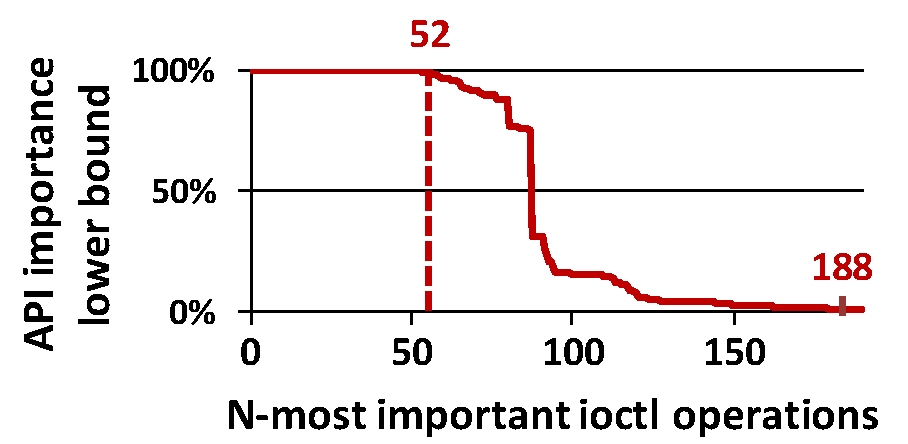
\includegraphics[width=.48\textwidth]{ioctl-popularity-by-inst.pdf}
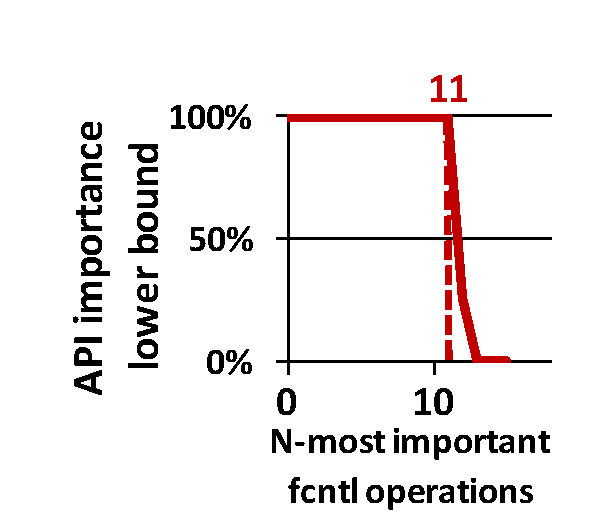
\includegraphics[width=.25\textwidth]{fcntl-popularity-by-inst.pdf}
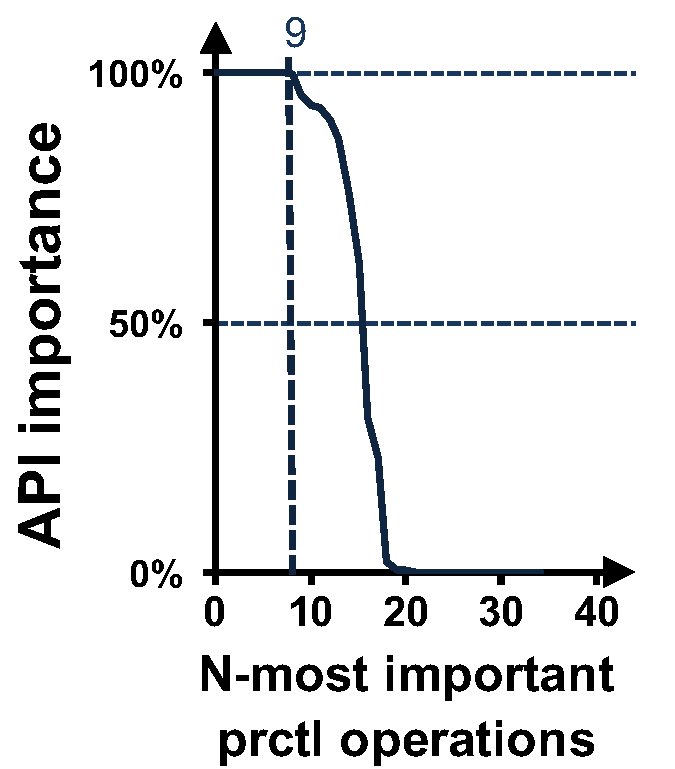
\includegraphics[width=.25\textwidth]{prctl-popularity-by-inst.pdf}
\caption{Ranking of \usagemetric{} among {ioctl}, {\tt fcntl} and {\tt prctl} opcodes.  Higher is more important; 100\% indicates all installations include software that request the operations.}
\label{fig:syspop:opcode-popularity}
\end{figure}


%\fixmedp{If time, it would be nice to investigate these zero cases and make sure no one really uses them}

%\begin{figure}[t]
%\center{
%\includegraphics[width=0.95\linewidth]{figures/fcntl-popularity.pdf}
%}
%\footnotesize
%\caption{Ranking of \usagemetric{} among {\tt fcntl} commands.}
%\label{fig:fcntl-popularity}
%\end{figure}

%\begin{figure}[t]
%\center{
%\includegraphics[width=0.95\linewidth]{figures/prctl-popularity.pdf}
%}
%\footnotesize
%\caption{Ranking of \usagemetric{} among {\tt prctl} codes.}
%\label{fig:prctl-popularity}
%\end{figure}

\section{Pseudo files and devices}
\label{sec:study:files}

In addition to the main system call table, Linux exports many additional APIs through 
pseudo-file systems, such as {\tt /proc}, {\tt /dev}, and {\tt /sys}.
These are called pseudo-file systems because they are not backed by disk, but
rather export the contents of kernel data structures to an application or administrator
as if they were stored in a file.
These pseudo-file systems are a convenient location to export tuning parameters, statistics, 
and other subsystem-specific or device-specific APIs.
Although many of these pseudo-files are used on the command line or in scripts by an administrator,
a few are routinely used by applications.
% interfaces are often the last resort of APIs, for accommodation of the most exotic interfaces. 
In order to fully understand usage patterns of the Linux kernel, pseudo-files must also be considered.

We apply static analysis to find cases where the binary is hard-coded to use a pseudo-file.
Our analysis cannot capture cases where a path to one of these file systems is passed as 
an input to the application, such as {\tt dd if=/dev/zero}.
However, when a pseudo-file is widely-used as a replacement for a system call,
these paths tend to be hard-coded in the binary as a string or string pattern.
%most instances of these file systems as system call replacements have hard-coded paths or patterns 
%in the binary.  
A common pattern we observed was {\tt sprintf(``/proc/\%d/cmdline'', pid)}; our analysis captured these patterns as well.
We also do not differentiate types of access in this study, such as separating read
versus write of a pseudo-file; rather we only consider whether the file is accessed or not.
Thus, our analysis is limited to strings stored in the binary, but we believe this captures
an important usage pattern.  %is a reasonable sample.


%% Note that matching hard-coded paths in binaries does not differentiate
%% the type of access on the files or devices.
%% The possible access on a pseudo file includes reading or writing data, retrieving file attributes, waiting on file descriptor events,
%% or performing directory operations.
%% Our study treat all access to one particular pseudo-file or device
%% as using the same API.

\begin{figure}[t]
\centering
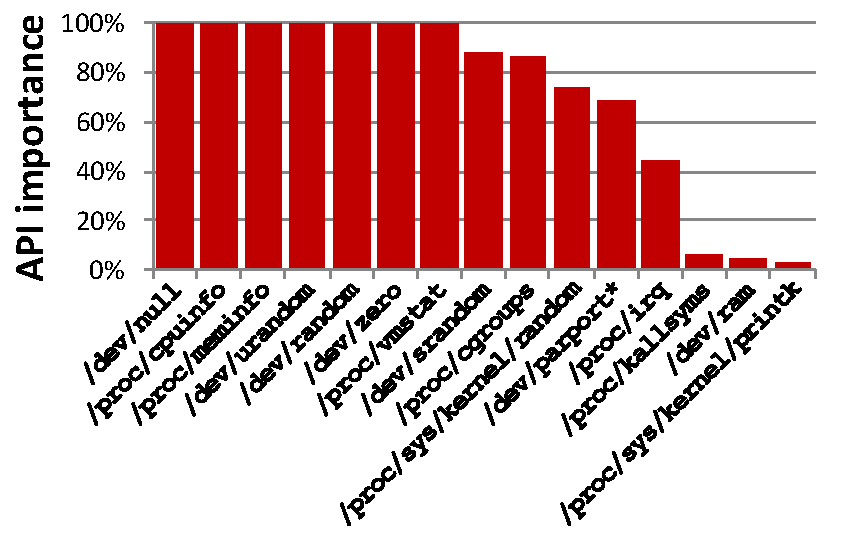
\includegraphics[width=5.5in]{dev-proc-popularity-by-inst.pdf}
\caption{\usagemetric{} distribution over files under {\tt /dev} and {\tt /proc}.  Higher is more important; 100\% indicates all installations include software that accesses the file. }
\label{fig:syspop:dev-proc-popularity}
\end{figure}

Figure~\ref{fig:syspop:dev-proc-popularity} shows the \usagemetric{} of common pseudo-files under {\tt/dev} and {\tt /proc}.  
These files are ordered from highest \usagemetric{}; the long tail
of files used rarely or directly by administrators is omitted.

%There are two striking facets of this data.
Some files %under {\tt /proc} and {\tt /dev}
are essential,
such as {\tt /dev/null} and {\tt /proc\-/\-cpuinfo}.
These files are widely used in %are hard to deprecate because the usage of
%these APIs exists in not only 
binaries and scripts.
%\fixmedp{Can we comment on how many apps or libraries include a hard-coded string or pattern?}
Among 12,039 binaries that use a hard-coded path,
3,324 access {\tt /dev/null} and 439 access {\tt /proc/cpuinfo}.
However, it is plausible to provide the same functionality in
simpler ways.
For instance, {\tt /proc/cpuinfo} provides a formatted wrapper for
the {\tt cpuinfo} instruction, which one could export
directly to userspace using virtualization hardware, similar to Dune~\citep{belay12dune}.
Similarly, {\tt /dev/zero} or {\tt /dev/null} are convenient for use on the command
line, but it is surprising that a significant number of applications
issue {\tt read} or {\tt write} system calls, rather than simply zeroing a buffer
or skipping the {\tt write}
(e.g., {\tt grub-install}).
%\fixmedp{Can we offer concrete examples of apps that do this?}
Thus, in implementing a Linux compatibility layer, a small number of pseudo-files
are essential, and perhaps others could be eliminated with modest application changes.


%% provide more security-aware alternatives
%% to these APIs, so security-sensitive applications
%% can remove the usage to reduce their attack surfaces.}
%% %These system calls can be either repromoted to system call interfaces,
%% %or directly served inside system libraries using a library OS approach,
%% %to avoid increasing API footprint.
%% For example, \libc{} can encapsulate {\tt /dev/null} and serve it in the user space.
%% %without the usage of real system calls.
%% {\tt /proc/cpuinfo} can be stored as a static information in user's memory,
%% or retrieved from CPU using the {\tt CPUINFO} instruction.

APIs as pseudo-files or pseudo-devices also have a large subset
of infrequently used or unused APIs.
%Second, pseudo-file systems contain a large collection of APIs that are infrequently used,
Many of them
are designed to support one specific application or user.
%only serve certain special purposes for few applications or end-users
For example, {\tt /dev/kvm} is only intended for {\tt qemu} to
communicate with the kernel portion of the KVM hypervisor.
Similarly {\tt /proc/kallsyms} is used primarily to export debugging information to kernel developers.

Because so many files in {\tt /proc} are accessed from the command line
or by only a single application, it is hard to conclude that any should be deprecated.
Nonetheless, these files represent large and complex APIs that create an important attack surface to defend.
As noted in other studies, the permission on {\tt /proc} tend to be
set liberally enough to leak a  significant amount of information~\citep{memento}.
%\fixmedp{Can we comment on how many of these are really accessible from regular applications/ how used in SELinux/AppArmor}
For files used by a single application, an abstraction like a fine-grained capability~\citep{shapiro99eros}
might better capture this need.  
%\fixmedp{I think kvm actually does use some sort of capability already. Please check.}
For files used primarily by the administrator,
carefully setting directory permissions should be sufficient.
%, but with careful consideration of using any security-enhanced Linux variant.



%% Although cleaning up the unused APIs is beneficial for the cleanness of the system design,
%% because pseudo-files and pseudo-devices are often considered
%% the last resort of APIs,
%% developers may choose not to deprecate them.
%% %there is no reason to deprecate them or delegate them to other interfaces
%% %if OS maintainers still consider the APIs useful.
%% %For example, {\tt /proc/kallsyms}
%% %only has \usagemetric{} less then ten percent,
%% %but it is
%% %a necessary API for Linux kernel development.
%% Instead of deprecating unused API,
%% we can apply more secure mechanisms, such as AppArmor or SELinux,
%% to restrict the access to particular applications.}
%% %to prevent them from becoming system vulnerabilities. 

%\callout{A few pseudo-files are essential and must be implemented
%by any Linux-emulator.  Most serve a specific purpose, and might benefit
%from stricter enforcement of the principle of least privilege.}

%For pseudo-files and devices that are ubiquitously important, system developers should provide more secure alternatives
%if possible. Infrequently used APIs that are important for particular applicatins need to be further secured.}}

%First, the \usagemetric{} of these file under {\tt /proc} is very bimodal.
%There are over 1,000 files that are not directly used by any application; we expect that most of these
%are interfaces for an administrator to adjust kernel behavior.

%Second, there are 148 files with an \usagemetric{} score above 90\%---almost as many as there are system calls with a similar \usagemetric{} score.

%\fixme{Remove the discussion about performance impact for now. Will resurrect it after I confirm it is true.}
%In some cases, libraries or applications can tolerate a missing {\tt /proc} file
%by falling back to default values or alternate interfaces.
%For instance, {\tt gcc} will try to read {\tt /proc/cpuinfo} to guide its selection of optimizations and {\tt /proc/meminfo} to avoid
%swapping; if this file is not available, 
%{\tt gcc} will use default values.
%Our static analysis does not detect these cases.
%Nonetheless, in building a Linux-compatibility system, whether these pseudo-files are accurately 
%emulated can have a first-order impact on performance.
%In our experience building the Graphene library OS~\citep{tsai14graphene}, {\tt gcc}
%performance \fixmedp{data nugget here}.

%developers interested in emulating Linux or similar systems should carefully evaluate their emulation of {\tt /proc}.

In the case of the {\tt /dev} file system, the most commonly used files are pseudo-devices, such as accessing
the virtual terminal ({\tt /dev/tty}, {\tt /dev/console}, and {\tt /dev/pts}), or other functionality 
such as the random number generator ({\tt /dev/urandom}).
Even among pseudo-devices, features such as accessing one's standard in and out, or a process's TTY
via the {\tt /dev/} interface are not heavily used.

Intuitively, one would not expect many device paths to be hard-coded, and most direct interactions 
with a device would be done using administrative tools.
For instance, we see that some applications do hard-code paths like {\tt /dev/hda} (commonly used for an IDE hard drive),
yet an increasing number of systems have a root hard drive using SATA, which would consequently be named {\tt /dev/sda}.
Thus, although applications may use paths like {\tt /dev/hda} as a default device path, modern systems are sufficiently varied
that these generally need to be searched at runtime.

%\begin{figure}[t]
%\centering
%\includegraphics[width=0.9\linewidth]{figures/sys-popularity.pdf}
%\caption{\usagemetric{} distribution over the set of files under {\tt /%sys}.  Higher is more heavily used; 1 indicates all systems include %software that accesses the file. }
%\label{fig:sys-popularity}
%\end{figure}

%In the case of {\tt /sys} (Figure~\ref{fig:sys-popularity}), 
%we again note that there are 63 paths with a \usagemetric{} value above 90\%,
%and a total of 97 above 20\%.  Several of these export CPU or power management features,
%or user-accessed buses, like USB.  Unlike {\tt /dev}, several of these hard-coded files 
%are also actual (expected) devices, such as PCMCIA devices.

%Table~\fixmedp{XX} lists the {\tt /proc} files with a \usagemetric{} score of one.  
%\fixmedp{What else to say about this?  Might be more interesting to know how ubiquitously used these are}

\section{C library APIs}
\label{sec:study:libc}

In addition to studying kernel interfaces, we also analyze the \usagemetric{} of APIs
defined in core system libraries, such as \libc{}.
Most programmers don't directly use the APIs exported by the kernel,
but instead program to more user-friendly APIs in \libc{} and other libraries.
%The \libc{} implementation contains lots of wrappers,
%or more user-friendly API variants of system calls and others.
For instance, \glibc{}~\citep{glibc} exports APIs for using locks and condition variables, which internally 
use the subtle {\tt futex} system call~\citep{franke02futex}.

%Figure~\ref{fig:syspop:libc-popularity} 
Our result shows that among %shows the \usagemetric{} of 
the global function symbols exported by 
\libc{} --- 1,274 in total % API among all packages. 
%Here we define \libc{} API as functions that are exported as global function symbols in \libc{}.
%The definition yields a total of 1,274  APIs,
%Among these APIs,
--- 42.8\% have a \usagemetric{} of 100\%,
50.6\% have a \usagemetric{} of less than 50\%,
and 39.7\% have a \usagemetric{} of less than one percent, including some that are not used at all.
In other words, about 40\% of the APIs inside \libc{}
are either not used or only used by few applications.
This result implies that most processes are loading a significant amount of 
unnecessary code into their address space.
By splitting \libc{} into several sub-libraries, based on \usagemetric{}
and common linking patterns, systems could realize a non-trivial space savings.

%\fixmedp{Can we assert that important and unimportant APIs are interleaved
%  on the same pages, so lazy loading doesn't help?}
There are several reasons to avoid loading extra code into an application.
First, there are code reuse attacks, such as return-oriented programming (ROP)~\citep{return-oriented},
that rely on the ability to find particular code snippets, called gadgets.
Littering a process with extra gadgets offers needless assistance to an attacker.
Similarly, when important and unimportant APIs are on the same page,
memory is wasted.  
Finally, the space overhead of large, unused jump tables is significant.
In \glibc{} 2.21, {\tt libc-2.21.so} essentially has 1274 relocation entries, occupying 30,576 bytes of virtual memory. 
%\fixmedp{true?: Because important and unimportant APIs are interleaved, all of these pages typically demand-allocated, even for applications that only use the most popular entries.}
By sorting the relocation table according to API usage,
most \libc{} instances could load only first few pages of relocation tables, and leave the remaining relocation entries for lazy loading.

We analyzed the space savings of a 
\glibc{} 2.21 which removed any APIs with \usagemetric{} lower than 90\%.
In total, \libc{} would retain 889 APIs
and the size would be reduced to 63\% of its original size.
%to \libc\_minor (in total  will stay in \libc{}).
%The size of \libc{} is reduced to 
The probability an application would need a missing function and load it from another library is less than 9.3\%(equivalent to 90.7\% \compatmetric{} for the stripped \libc{}).
%and the probability of any application loading \libc\_minor is smaller than 9.3\% 
Further decomposition is also possible, 
such as placing APIs
that are commonly accessed by the same application into the same sub-library.

%% Knowing the usage of \libc{} APIs, developers can decompose
%% a large \libc{} binary into smaller libraries.
%% Breaking down the size of \libc{} binary effectively reduces
%% the security threats in \libc{},
%% such as the risk of ROP (Return-Oriented Programming) attack.
%% The simplest way of decomposing \libc{} is
%% to move all APIs with lower \usagemetric{}
%% to another library \libc\_minor.


%It could reduce effective memory footprint to deprecate the functions that are never used, 
%or move rarely-used APIs into a separate library. % additional libraries so they do not have to be loaded or installed all the time.

%% \rev{Transition}{Another minor benefit of decomposing \libc{}
%% or just re-ordering \libc{} APIs
%% is to optimize the resource usage needed for dynamic loading of these APIs.}
%% %Other usage of this statistics is to provide them to compilers as a hint to optimize the dynamic loading.
%% Dynamic libraries like \libc{} are relocated during loading time
%% of user processes,
%% and the virtual memory used for storing relocation tables for
%% all libraries loaded in all user processes can be a non-trivial memory footprint because they are unable to share physical pages.
%% In \glibc{} 2.21, {\tt libc-2.21.so} essentially has 1274 relocation entries, occupying 30,576 bytes of virtual memory. 
%% By sorting the relocation table according to API usage,
%% Most \libc{} can load only first few pages of relocation tables, and leave the remaining relocation entries for lazy loading.

%\callout{Decomposing or re-ordering library API can lower memory costs
%in typical application processes.}
%API usage statistics are hints for compilers to optimize memory footprint of dynamic loading by sorting relocation tables by \usagemetric

%\begin{figure}[t]
%\centering
%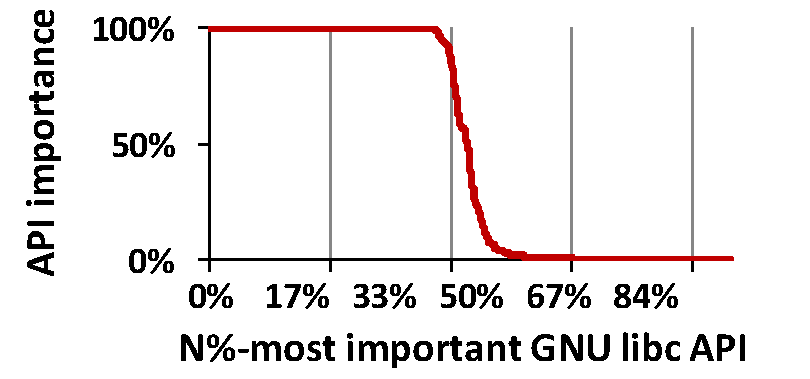
\includegraphics[width=3.6in]{syspop/figures/libc-popularity.pdf}
%\caption[\Usagemetric{} distribution of GNU Library C functions]
%{\usagemetric{} distribution over the set of GNU Library C. Higher is more important; 100\% indicates all installations include software that use the \libc{} API. }
%\label{fig:libc-popularity}
%\end{figure}

%%%We observe that majority (xx \%) of the executables in the \osdist{} repository are ELF binaries (Figure~\ref{fig:executable-type}).
%%%The other executables rely on interpreters like shell, perl, python, etc. We focus our study
%%%only on the ELF binaries which also include the interpreters for other scripts. However, we do
%%%not use the scripts popularity and their footprint while calculating the metric for system call popularity.
%%%Overall, in order to get a compatibility score with Linux for any given OS, we calculate popularity of 4 different
%%%interfaces that the applications use.

\paragraph{Effects of standard libraries on \usagemetric{}.} \Libc{} and the dynamic linker ({\tt ld.so}) 
also contribute to the system call footprint of every dynamically-linked executable.
This has a marked effect on the \usagemetric{} of some system calls.
The APIs used to initialize a program  are listed in Table~\ref{table:libc-init-call}.
In several cases, such as {\tt set\_tid\_address}, however, \libc{} or \libpthread{} may be the only binaries using these interfaces directly,
indicating that changes to some important system interfaces would only require changes in one or two low-level libraries.

%\callout{GNU Library C and the dynamic linker can have a first-order effect on the \usagemetric{} of some system calls.}

%%% \begin{compactenum}
%%% \item Users and developers are often unaware of the footprint caused inside initialization and finalization of \libc{}. For library APIs, users at least have basic sense about what the footprint may look like.
%%% \item It requires only minimal effort to maintain compatibility between GNU Library C and kernel, because the development is actually closely coupled. 
%%% \end{compactenum}
 

%%% These APIs are also the fundamental API footprint of a {\tt Hello World} program.
%%% The developers of GNU C library made the choice of relying on certain APIs, making them one of the most important in the system. 

%%% For example, in our study, the usage in \libc{} has increased the \usagemetric{} of system call {\tt set\_tid\_address} by 0.75, suggesting that deprecating the system call will takes only little effort but changing {\em libc} itself.    

\begin{table}[t]
\centering
\small
\begin{tabular}{>{\footnotesize\raggedright\arraybackslash}m{.6\textwidth}>{\raggedright\arraybackslash}m{.3\textwidth}}
\hline
\addlinespace
System Calls & Libraries \\
\addlinespace
\hline
{\tt access}, {\tt arch\_prctl}, {\tt mprotect} & ld.so \\
\hline
{\tt clone}, {\tt execve}, {\tt getuid}, {\tt gettid},
{\tt kill}, {\tt getrlimit}, {\tt setresuid} & libc \\
\hline
{\tt close}, {\tt exit}, {\tt exit\_group}, {\tt getcwd},
{\tt getdents}, {\tt getpid}, {\tt lseek}, {\tt lstat},
{\tt mmap}, {\tt munmap}, {\tt madvise}, {\tt mprotect},
{\tt mremap}, {\tt newfsstat}, {\tt read} &
libc, ld.so \\
\hline
{\tt rt\_sigreturn}, {\tt set\_robust\_list}, {\tt set\_tid\_address} &
libpthread \\
\hline
{\tt rt\_sigprocmask} &
librt \\
\hline
{\tt futex} &
libc, ld.so, libpthread \\
\hline
\end{tabular}
\footnotesize
\caption{Ubiquitous system call usage caused by initialization or finalization of \libc{} family.}
\label{table:libc-init-call}
\end{table}
